\documentclass[12pt]{article}
% Margin fixes
\oddsidemargin -0.5in
\evensidemargin -0.5in
\textwidth 7.25in
\topmargin 0.0in

\headheight 0.0pt
\headsep 0.0pt
\voffset 0.0pt
\textheight = 9.0in
\usepackage{amsmath,amssymb,graphicx,float}

\title{Nuclear Spectroscopy}
\author{Nathan Grouse\\Lisa Tran}

\newcommand{\eV}{\text{eV}}
\newcommand{\V}{\text{V}}
\newcommand{\A}{\text{A}}

% Start the document!
\newcommand{\documentname}{\textsl{Article}}
\begin{document}
\maketitle

\section{Introduction}
\indent \indent The purpose of this lab is to measure and interpret the energy distrubitions of particles emitted by radioactive nuclei.

\subsection{Apparatus}
\indent \indent A detector, scintillartor (contained by the detector), photomultiplier (contained), high voltage power supply, multi-channel analyzer or MCA box, Sensor-CASSY, and lead bricks are used.

\begin{figure}[H]
\centering
\hspace{-0.0in}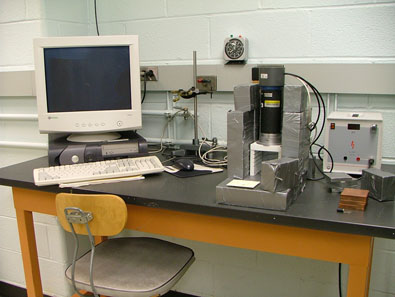
\includegraphics[scale=0.90]{apparatus.png}
\end{figure}

\section{Theory}
\indent \indent The first bits of theory are detailed qualitative explainations of different types of radiation. \\
\indent The energy loss per differential length, caused by ionization and excitation, of charged particle radiation:
\[\frac{dE}{dx} \propto \frac{z^2e^2NZ}{mV^2} ,\]
\indent where z times e is the charge of the particle, N is the number density of the absorber, Z is the atomic number of the absorber, m is the mass of the electron, and V is the speed of the particle. This seems reasonable in that the faster moving partcles lose less energy over a fixed path length. It's also reasonable to say a more strongly charged particle would be more affected by the absorber and lose more energy in collisions - the rate of which increases as density and atomic number of the absorber increase. \\

\indent The last section of the lab gives the emerging intensity of a beam of mono-energetic gamma rays of intensity $I_0$ incident normally on a plane with thickness x:
\[I = I_0 e^-^\mu^x , \]
\indent where $\mu$ is the linear attentuation coefficent, which is kind of like absorption in that attentuate occurs when there is flux through a medium. The thicker the material, the greater the reduction of initial intensity.

\section{Data}
\begin{figure}[H]
\centering
\hspace{-0.0in}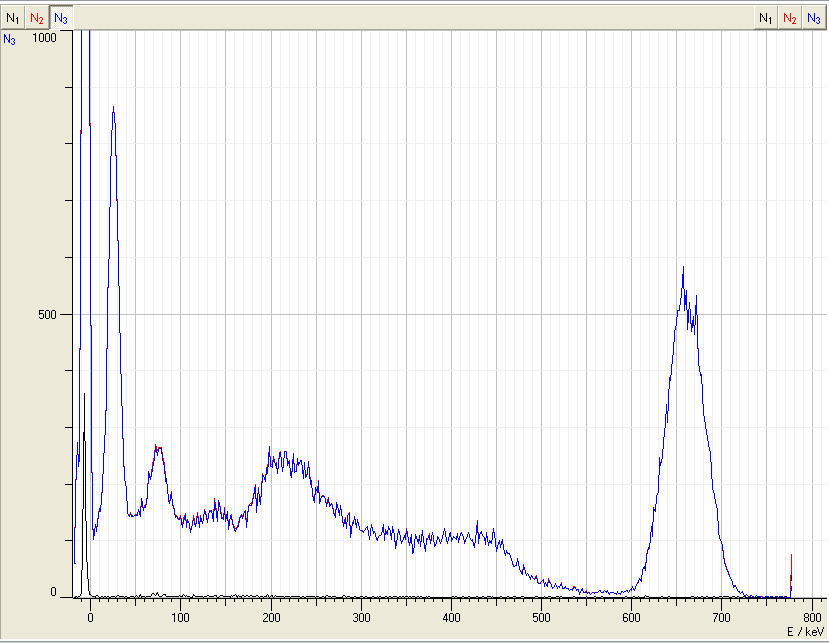
\includegraphics[scale=0.60]{Plot1.png}
\caption{Cesium-137 Radiation \label{fig:setup}}
\end{figure}

\begin{figure}[H]
\centering
\hspace{-0.0in}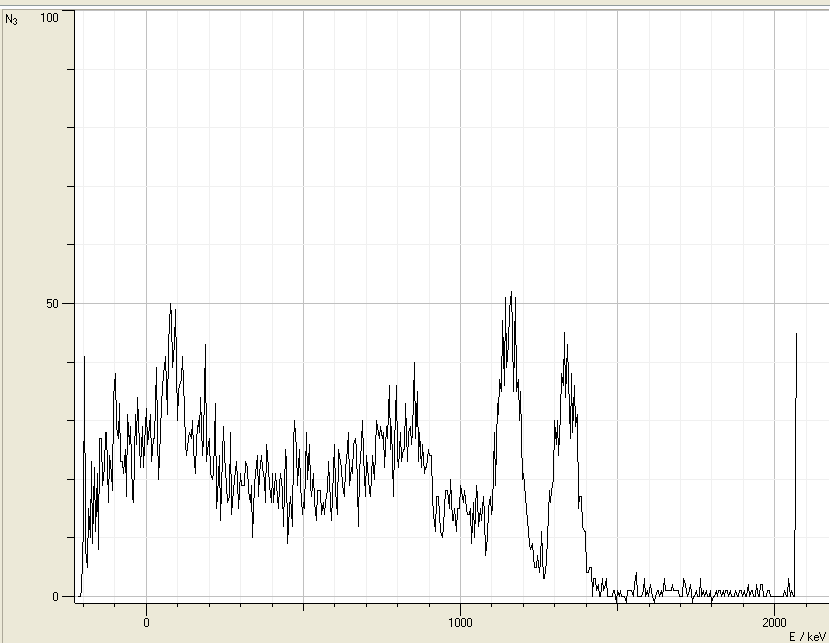
\includegraphics[scale=0.60]{Plot2.png}
\caption{Cobalt-60 Radiation \label{fig:setup}}
\end{figure}

\begin{figure}[H]
\centering
\hspace{-0.0in}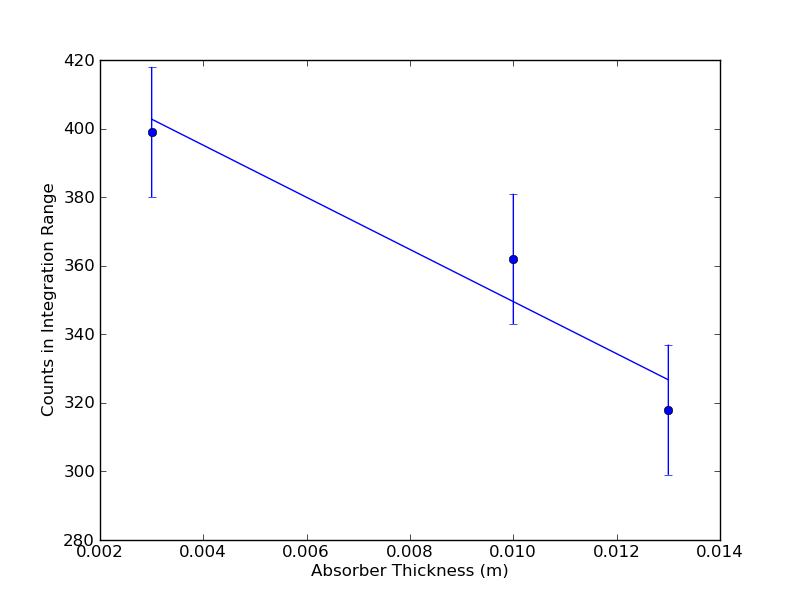
\includegraphics[scale=0.60]{Plot3.png}
\caption{Aluminum \label{fig:setup}}
\end{figure}

\begin{figure}[H]
\centering
\hspace{-0.0in}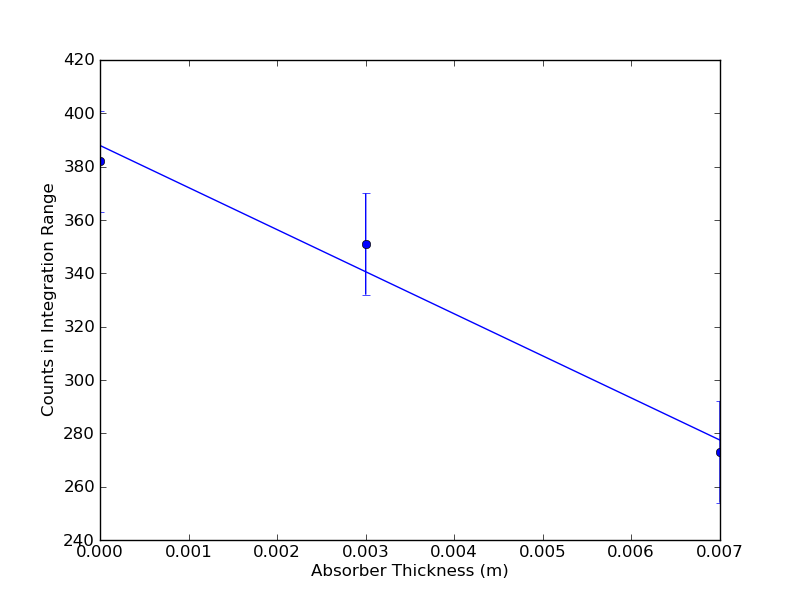
\includegraphics[scale=0.60]{Plot4.png}
\caption{Copper \label{fig:setup}}
\end{figure}

\begin{figure}[H]
\centering
\hspace{-0.0in}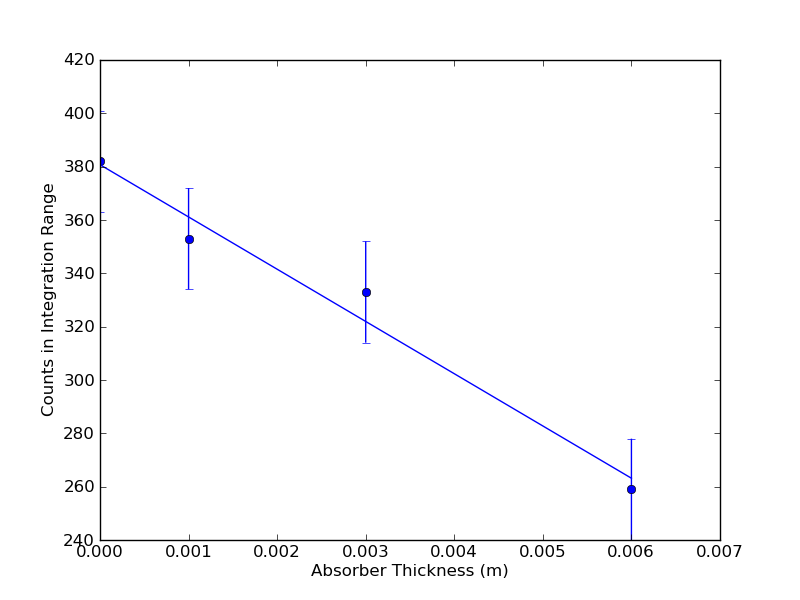
\includegraphics[scale=0.60]{Plot5.png}
\caption{Lead \label{fig:setup}}
\end{figure}

\section{Calculations}
\[\mu_a_l = -7601 \frac{1}{m} \]
\[\mu_c_u = -15784 \frac{1}{m} \]
\[\mu_p_b = -19595 \frac{1}{m} \]
\indent The $\mu$ values are all negative because the slope of the line fit actually is negative. The given equation is a decreasing exponential because it's clear that absorbers will decrease the intial intensity.

\section{Error Analysis}
\indent \indent Uncertainty in the detector:
\[\delta q = \sqrt{N_0} = \sqrt{382} = 19 . \]

\indent Any naturally occuring backround radiation in the room will affect the results of this experiment. Lead bricks do a good job of reducing the background.

\section{Conclusion}
\indent \indent I saw everything I expected to see for the Cesium energy distribution. For the Cobalt spectrum: The peaks at about 1.17 MeV and 1.33 MeV correspond to the total absorption peak for Cobalt. Since Ni goes to ground state by emitting two gamma rays, there should be two compton edges. One edge is probably at about 870 keV because there is a sharp decline at about 900 KeV in detections and it is about 150 KeV less than the maximum for the lower energy total absorption peak. The other is probably around 1.2 MeV because that's about 150 KeV less than the maximum of the higher energy absorption peak and the total absorption peak for the 1.17 MeV gamma ray has N more counts than the other peak, where N is approximately the number of counts for the higher energy compton edge. Higher and lower energy electrons correspond to the gamma rays emitted by Nickel. The lower maximum energy of backscatter photons is about 550 KeV and the higher maximum energy is about 900 KeV, also corresponding with the discontinuity. Both of these values are about 300 KeV less than their respective compton edges.

\section{Questions}
\indent \indent 1. Is the plot pretty much a straight line? \\
\indent Yes. \\
\indent 2. How does the absorption coefficient depend on the mass density of the absorber? \\
\indent As the mass density increases so does the absorption coefficient. \\
\indent 3. How does the absoption coefficient depend on the energy of the gamma ray? \\
\indent We were running low on time for this part of the lab and only gathered data with the Cobalt source. \\
\indent I would guess that the absorption coefficient would decrease as the energy of the gamma ray
\indent increases.

\end{document}